\documentclass[pdf]{beamer}
\usetheme{CambridgeUS}
\definecolor{WiLabRed}{RGB}{197,18,48}
                               \setbeamercolor{frametitle}{fg=white,bg=WiLabRed}
\setbeamercolor{progress bar}{fg=WiLabRed!90}
\setbeamercolor{palette tertiary}{fg=white,bg=WiLabRed}
\setbeamercolor{title separator}{fg=WiLabRed!90}
\setbeamercolor{progress bar in section page}{fg=WiLabRed!90}
\setbeamercolor{background canvas}{bg=white}
\setbeamercolor{alerted text}{fg=WiLabRed!90}
\setbeamertemplate{headline}


\setbeamertemplate{footline}
{
  \leavevmode%
  \hbox{%
  \begin{beamercolorbox}[wd=.3\paperwidth,ht=2.25ex,dp=1ex,center]{author in head/foot}%
    \usebeamerfont{author in head/foot}Kyle W. McClintick
  \end{beamercolorbox}%
  \begin{beamercolorbox}[wd=.6\paperwidth,ht=2.25ex,dp=1ex,center]{title in head/foot}%
    \usebeamerfont{title in head/foot}Email: \Letter kwmcclintick@wpi.edu
  \end{beamercolorbox}%
  \begin{beamercolorbox}[wd=.1\paperwidth,ht=2.25ex,dp=1ex,center]{date in head/foot}%
    \insertframenumber{} / \inserttotalframenumber\hspace*{1ex}
  \end{beamercolorbox}}%
  \vskip0pt%
}

\usepackage{xcolor}
\usepackage{appendixnumberbeamer}
\usepackage{booktabs}
\usepackage{hyperref}
\usepackage{wrapfig}
\usepackage[scale=2]{ccicons}
\usepackage{pgfplots}
\usepgfplotslibrary{dateplot}
\usepackage{xspace}
\newcommand{\themename}{\textbf{\textsc{metropolis}}\xspace}
\graphicspath{{./Images/}{./Misc/}}
\usepackage{marvosym}
\usepackage{subfig}
\usepackage{graphicx}
\usepackage{verbatim}
\usepackage{caption}


\title{TrojDRL: Trojan Attacks on DeepReinforcement Learning Agents}
\date{April 29th, 2020}
\author{\textbf{Kyle McClintick} \small{\\ Dept. of Electrical \& Computer Engineering, Worcester Polytechnic Institute, Worcester, MA 01609 USA}}
\vspace{-20cm}
\institute{ \hfill
\includegraphics[height=1.5cm]{wilab_logo-A70916.eps}\hspace*{1.7cm}
\includegraphics[height=1.5cm]{WPI_Inst_Prim_FulClr.eps}}

\usepackage{csquotes}
\usepackage[style=verbose-ibid,backend=bibtex]{biblatex}
\bibliography{myreferences.bib}


\begin{document}

\captionsetup[subfigure]{labelformat=empty}

\maketitle







%%%%%%%%%%%%%%%%%%%%%%%%%%%%%%%%%%%%%%%%%%%%%%%%%%%%%%%%%%%%%%%%%%%%%%
\begin{frame}[fragile]{Personal Interest}
\begin{figure}
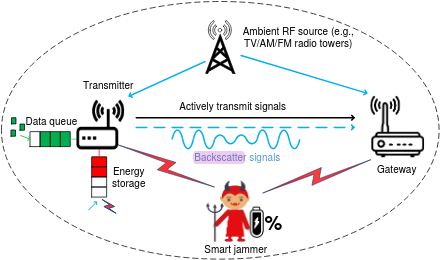
\includegraphics[width=0.7\linewidth,keepaspectratio]{Images/jam_if_can.png}
\caption{Small but growing community of people that believe DRL can lead to the development of a universal anti-jammer (2014-present). Earliest works funded by Air Force Research Labs (AFRL).}
\end{figure}
\end{frame}




%%%%%%%%%%%%%%%%%%%%%%%%%%%%%%%%%%%%%%%%%%%%%%%%%%%%%%%%%%%%%%%%%%%%%%
\begin{frame}[fragile]{Agenda}
\begin{minipage}[0.2\textheight]{\textwidth}
\begin{columns}[T]
\begin{column}{0.5\textwidth}
\begin{itemize}
\item Abstract
\item Key Contributions
\item Background
\item Novel Method
\item Results
\item Defense
\item Conclusion
\end{itemize}
\end{column}
\begin{column}{0.5\textwidth}
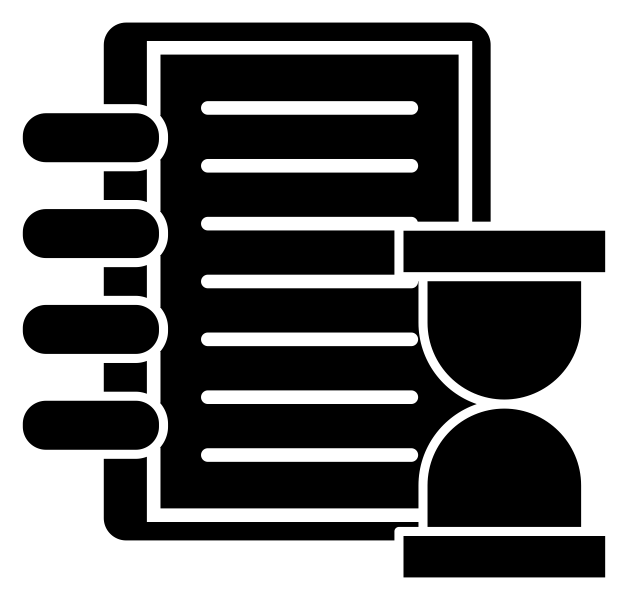
\includegraphics[width=5cm]{Images/agenda.png}
\end{column}
\end{columns}
\end{minipage}
\end{frame}




%%%%%%%%%%%%%%%%%%%%%%%%%%%%%%%%%%%%%%%%%%%%%%%%%%%%%%%%%%%%%%%%%%%%%%
\begin{frame}[fragile]{Abstract}
\begin{figure}
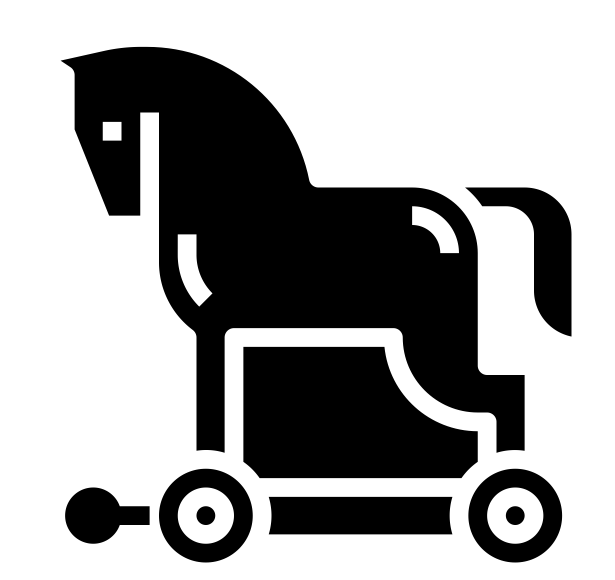
\includegraphics[width=0.3\linewidth,keepaspectratio]{Images/trojan.png}
\caption{Deep reinforcement learning (DRL) agents are weak to Trojan attacks that augment as little as 0.025\% of the training data. Existing defense mechanisms are not effective.}
\end{figure}
\end{frame}





%%%%%%%%%%%%%%%%%%%%%%%%%%%%%%%%%%%%%%%%%%%%%%%%%%%%%%%%%%%%%%%%%%%%%%
\begin{frame}[fragile]{Key Contributions}
\begin{minipage}[0.2\textheight]{\textwidth}
\begin{columns}[T]
\begin{column}{0.5\textwidth}
\begin{itemize}
\item TrojDRL: manipulating training data rewards
\item Vulnerabilities to Trojan attacks even when restricted to tampering with only training data states
\item Demonstrate that state-of-the-art defense mechanisms for Trojaned neural networks do not extend to the DRL case.
\end{itemize}
\end{column}
\begin{column}{0.5\textwidth}
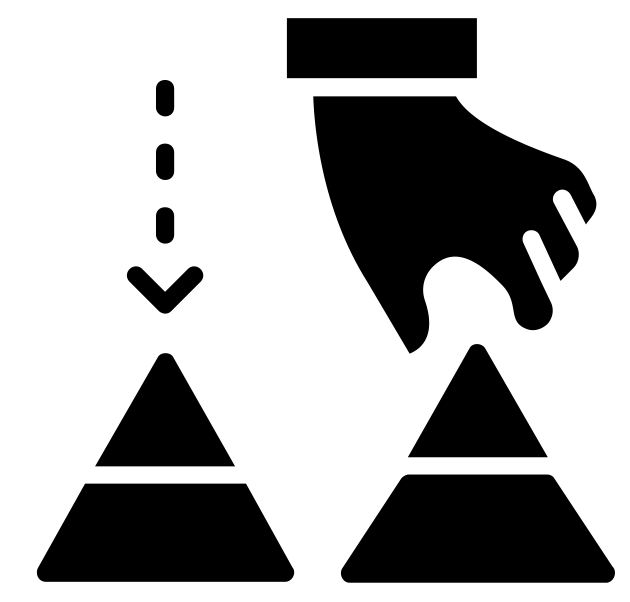
\includegraphics[width=5cm]{Images/contribute.png}
\end{column}
\end{columns}
\end{minipage}
\end{frame}







%%%%%%%%%%%%%%%%%%%%%%%%%%%%%%%%%%%%%%%%%%%%%%%%%%%%%%%%%%%%%%%%%%%%%%
\begin{frame}[fragile]{Background: Reinforcement Learning}
\begin{figure}
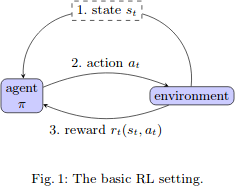
\includegraphics[width=.5\linewidth,keepaspectratio]{Images/drl.png}
\end{figure}
\end{frame}


%%%%%%%%%%%%%%%%%%%%%%%%%%%%%%%%%%%%%%%%%%%%%%%%%%%%%%%%%%%%%%%%%%%%%%
\begin{frame}[fragile]{Background: Trojan Backdoor Attacks}
\begin{figure}
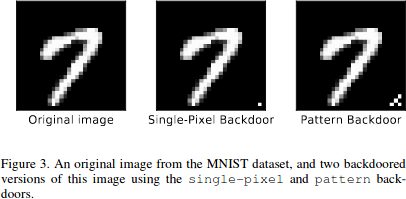
\includegraphics[width=.8\linewidth,keepaspectratio]{Images/backdoor.png}
\end{figure}
\end{frame}




%%%%%%%%%%%%%%%%%%%%%%%%%%%%%%%%%%%%%%%%%%%%%%%%%%%%%%%%%%%%%%%%%%%%%%
\begin{frame}[fragile]{Novel Method: Objective}
\begin{minipage}[0.2\textheight]{\textwidth}
\begin{columns}[T]
\begin{column}{0.5\textwidth}
Alter as few states as possible using pattern $\Delta$, mask $\lambda$:
\\
\vspace{.5cm}
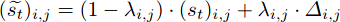
\includegraphics[width=6cm]{Images/state_poison.png}
\\
\vspace{.5cm}
Such that the triggered and untriggered policy have similar rewards when unactivated
\\
\vspace{.5cm}
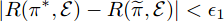
\includegraphics[width=4cm]{Images/obj1.png}
\\
\vspace{.5cm}
And maximally different rewards when activated:
\\
\vspace{.5cm}
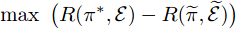
\includegraphics[width=4cm]{Images/obj2.png}
\end{column}
\begin{column}{0.5\textwidth}
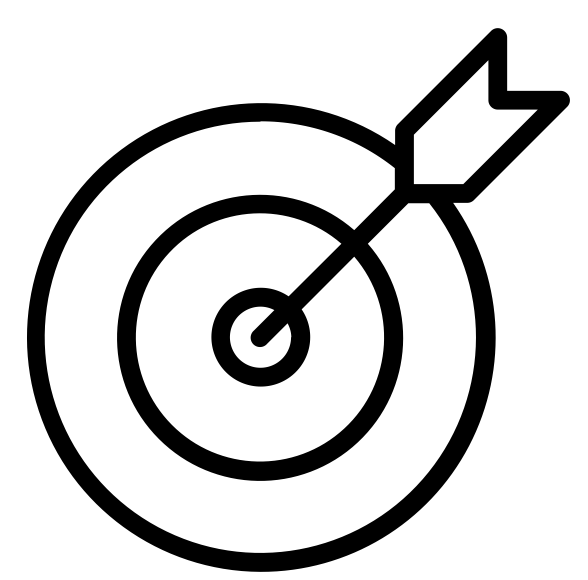
\includegraphics[width=5cm]{Images/obj.png}
\end{column}
\end{columns}
\end{minipage}
\end{frame}


%%%%%%%%%%%%%%%%%%%%%%%%%%%%%%%%%%%%%%%%%%%%%%%%%%%%%%%%%%%%%%%%%%%%%%
\begin{frame}[fragile]{Novel Method: Reward Hacking}
\begin{minipage}[0.2\textheight]{\textwidth}
\begin{columns}[T]
\begin{column}{0.5\textwidth}
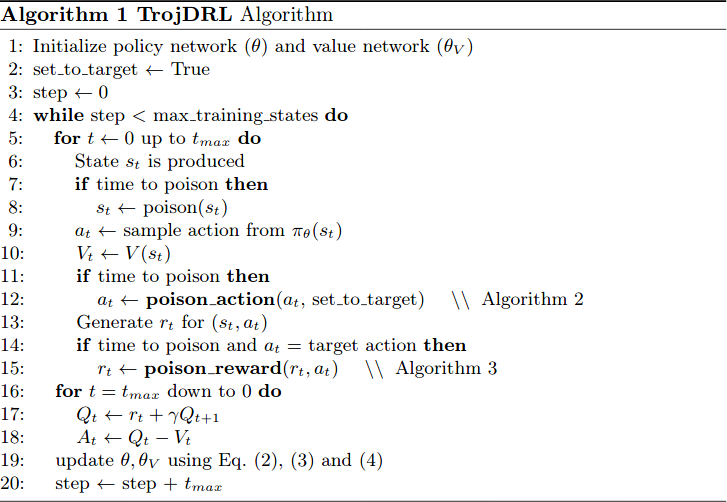
\includegraphics[width=10cm]{Images/alg1.png}
\end{column}
\begin{column}{0.3\textwidth}
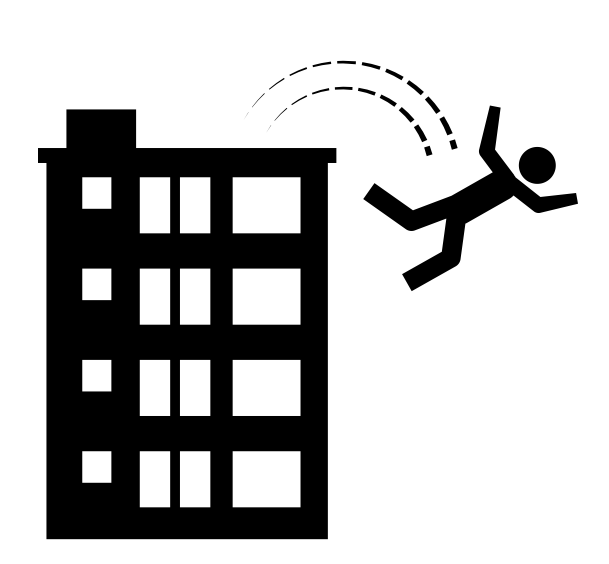
\includegraphics[width=4cm]{Images/rew_hack.png}
\end{column}
\end{columns}
\end{minipage}
\end{frame}



%%%%%%%%%%%%%%%%%%%%%%%%%%%%%%%%%%%%%%%%%%%%%%%%%%%%%%%%%%%%%%%%%%%%%%
\begin{frame}[fragile]{Novel Method: Data Representation}
\begin{minipage}[0.2\textheight]{\textwidth}
\begin{columns}[T]
\begin{column}{0.6\textwidth}
Experiments performed using Python Gym library:
\begin{itemize}
\item States: Atari game screens, $s_t \in \{0,...,255 \} ^{40,192,3}$. Games include Breakout, Pong, Qbert, Space Invaders, Seaquest and Crazy Climber
\item Actions: Up, down, left, right, fire, $a_t \in \{ 0,4 \}$
\item Reward: Vary by game. Good things typically get a reward $r_t = 1$, all else $r_t=0$. If game is time-sensitive, may instead be set to $r_t=\pm 1$.
\end{itemize}
\end{column}
\begin{column}{0.4\textwidth}
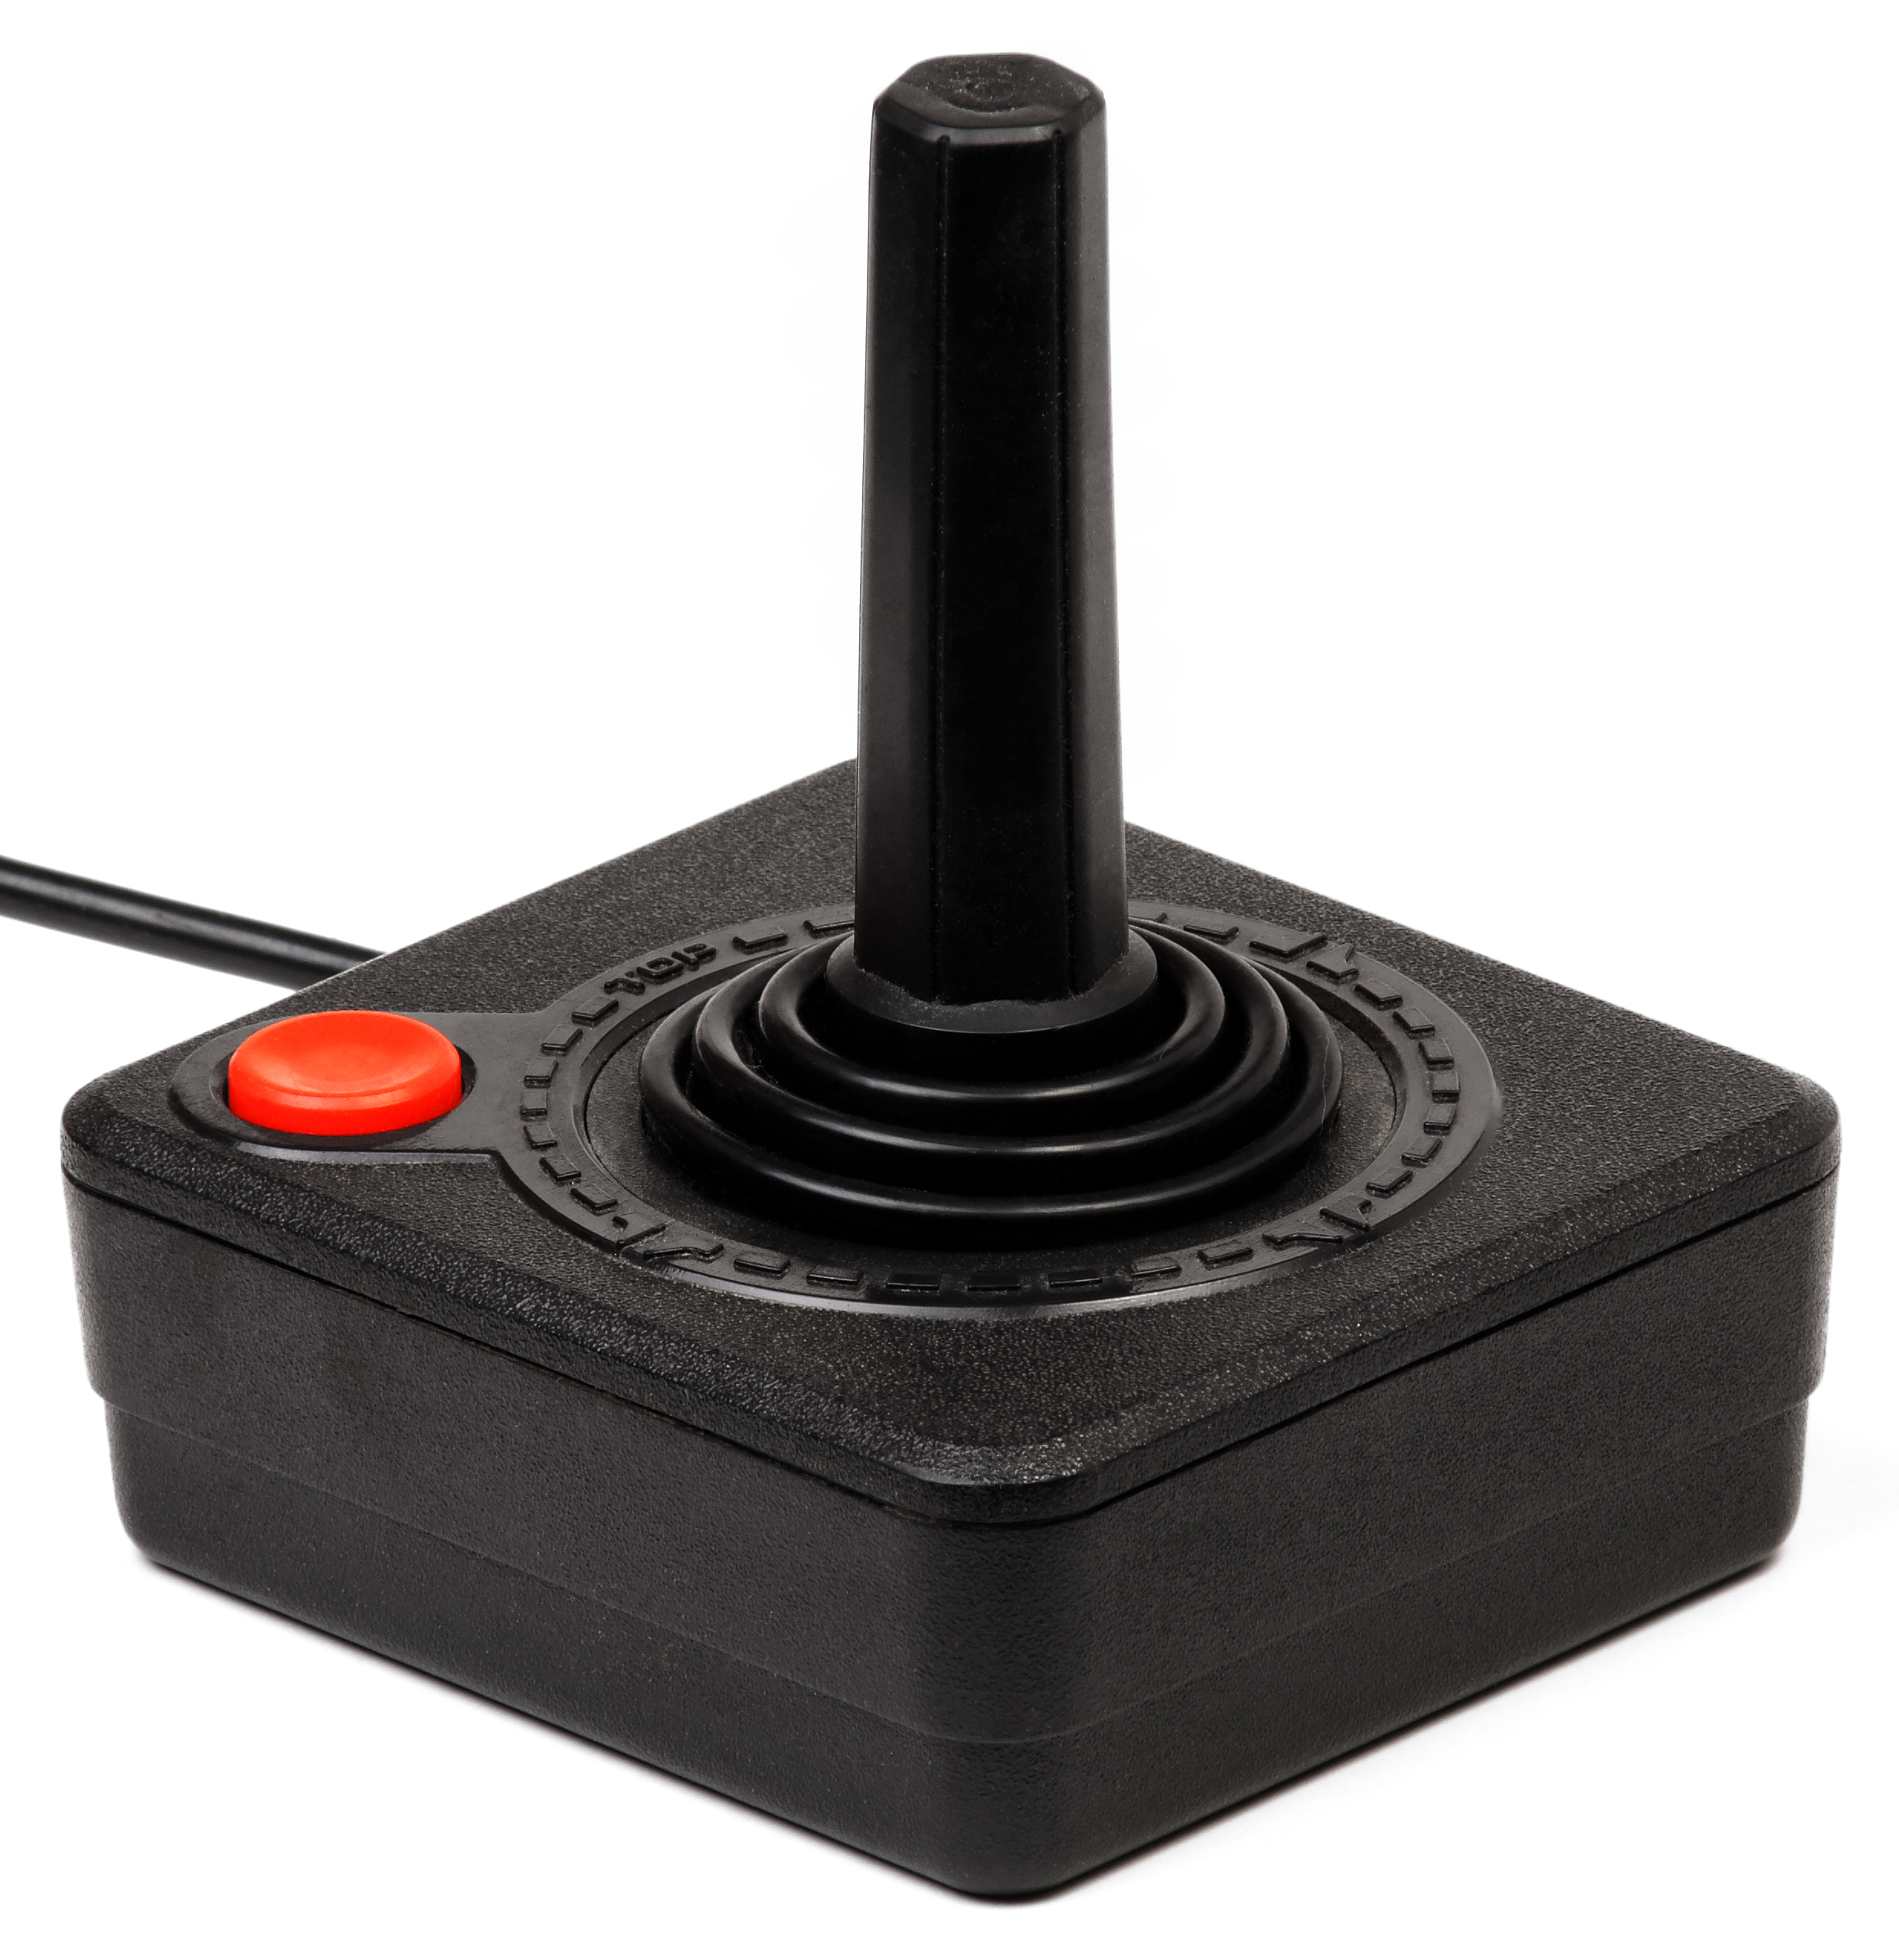
\includegraphics[width=4cm]{Images/atari.jpg}
\\
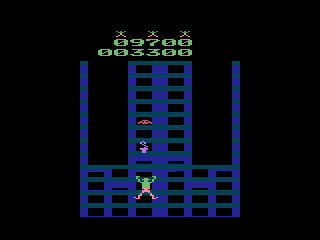
\includegraphics[width=4cm]{Images/crazy.png}
\end{column}
\end{columns}
\end{minipage}
\end{frame}





%%%%%%%%%%%%%%%%%%%%%%%%%%%%%%%%%%%%%%%%%%%%%%%%%%%%%%%%%%%%%%%%%%%%%%
\begin{frame}[fragile]{Results: Performance Gap}
\begin{figure}
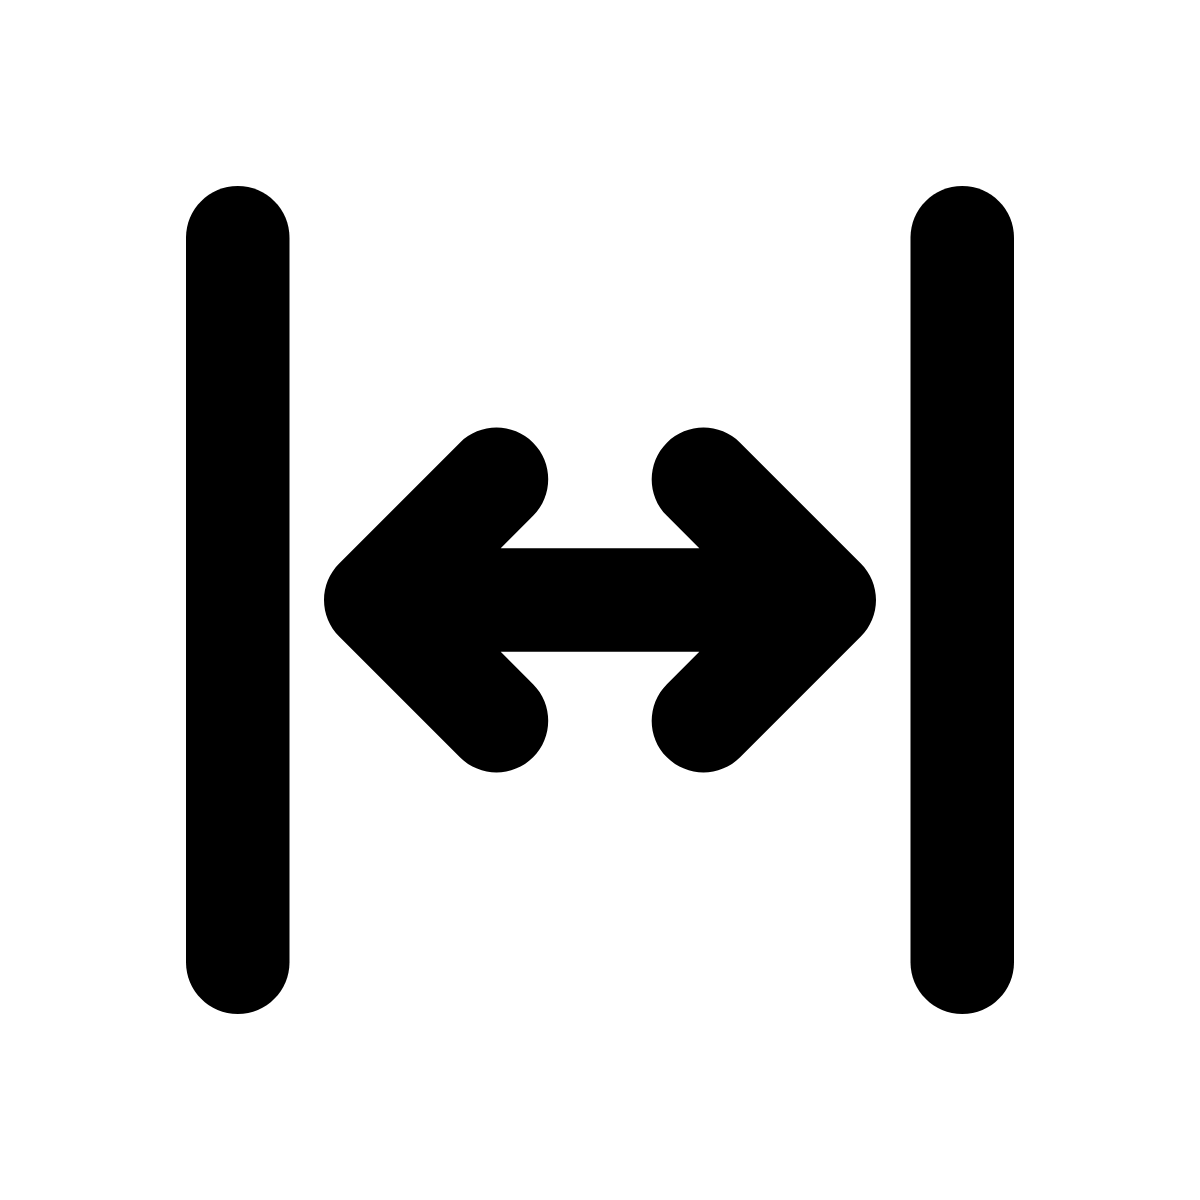
\includegraphics[width=0.2\linewidth,keepaspectratio]{Images/gap.png}
\\
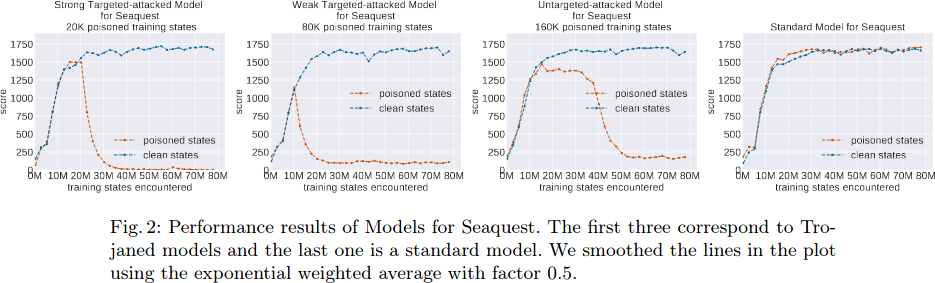
\includegraphics[width=1\linewidth,keepaspectratio]{Images/gap_plot.png}
\caption{20K out of 80M training states poisoned, which corresponds to poisoning only 0.025\%}
\end{figure}
\end{frame}

%%%%%%%%%%%%%%%%%%%%%%%%%%%%%%%%%%%%%%%%%%%%%%%%%%%%%%%%%%%%%%%%%%%%%%
\begin{frame}[fragile]{Results: Percentage of Target Action}
\begin{figure}
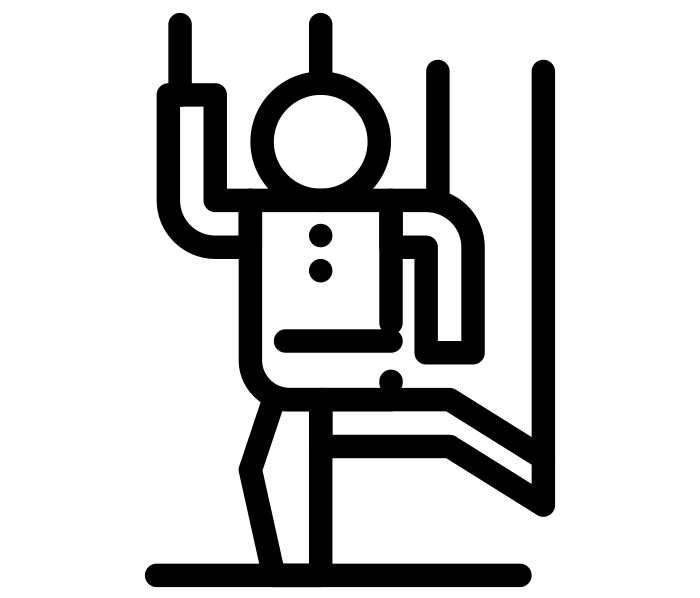
\includegraphics[width=0.2\linewidth,keepaspectratio]{Images/command.png}
\\
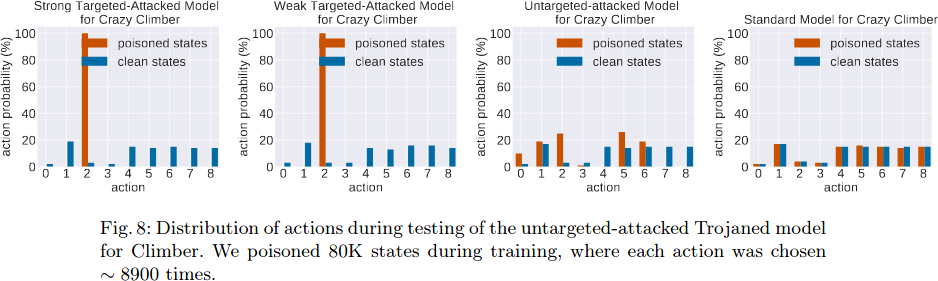
\includegraphics[width=1\linewidth,keepaspectratio]{Images/pota.png}
\end{figure}
\end{frame}


%%%%%%%%%%%%%%%%%%%%%%%%%%%%%%%%%%%%%%%%%%%%%%%%%%%%%%%%%%%%%%%%%%%%%%
\begin{frame}[fragile]{Resutls: Time to Failure}
\begin{figure}
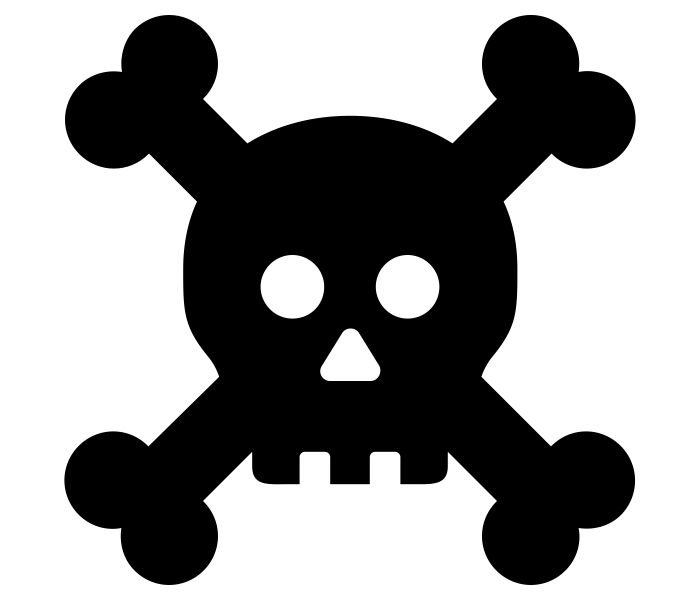
\includegraphics[width=0.2\linewidth,keepaspectratio]{Images/death.png}
\\
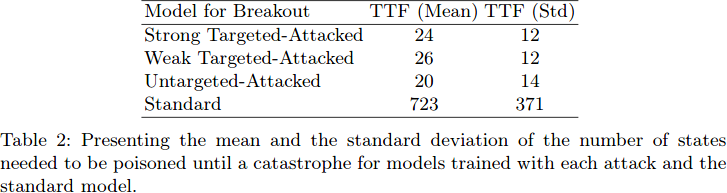
\includegraphics[width=1\linewidth,keepaspectratio]{Images/ttf.png}
\end{figure}
\end{frame}



%%%%%%%%%%%%%%%%%%%%%%%%%%%%%%%%%%%%%%%%%%%%%%%%%%%%%%%%%%%%%%%%%%%%%%
\begin{frame}[fragile]{Defense: Neural Cleanse}
\begin{figure}
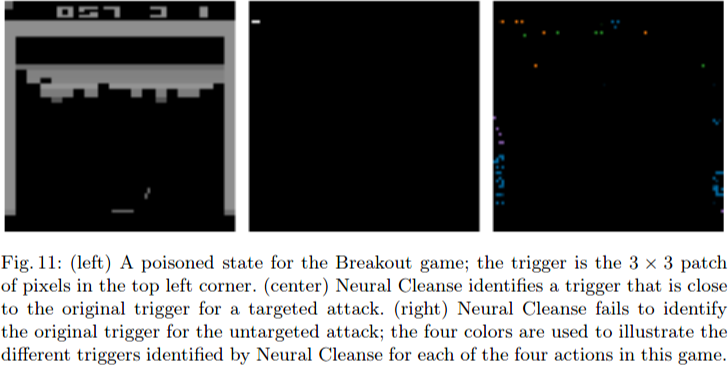
\includegraphics[width=1\linewidth,keepaspectratio]{Images/ncleanse.png}
\end{figure}
\end{frame}


%%%%%%%%%%%%%%%%%%%%%%%%%%%%%%%%%%%%%%%%%%%%%%%%%%%%%%%%%%%%%%%%%%%%%%
\begin{frame}[fragile]{Defense: Neural Cleanse}
\begin{minipage}[0.2\textheight]{\textwidth}
\begin{columns}[T]
\begin{column}{0.7\textwidth}
\begin{enumerate}
\item For a label, we design an optimization scheme to find the minimal trigger required to misclassify all samples from other labels into this target label
\item Repeat step 1 for each of $N$ output label in the model
\item After calculating $N$ potential triggers, measure the size of each trigger
\item Run an outlier detection algorithm to detect if any trigger candidate is significantly smaller than other candidates
\item Significant outlier represents a real trigger, and the label matching that trigger is the target label of the backdoor attack
\end{enumerate}
\end{column}
\begin{column}{0.2\textwidth}
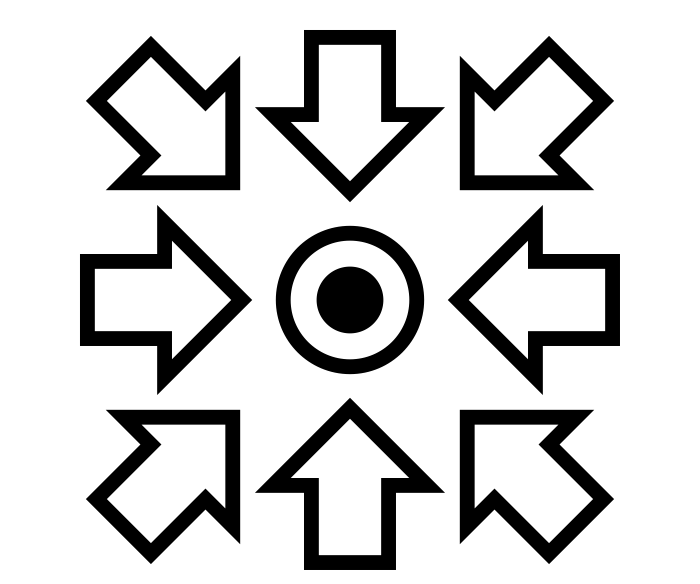
\includegraphics[width=1.8cm]{Images/1.png}
\\
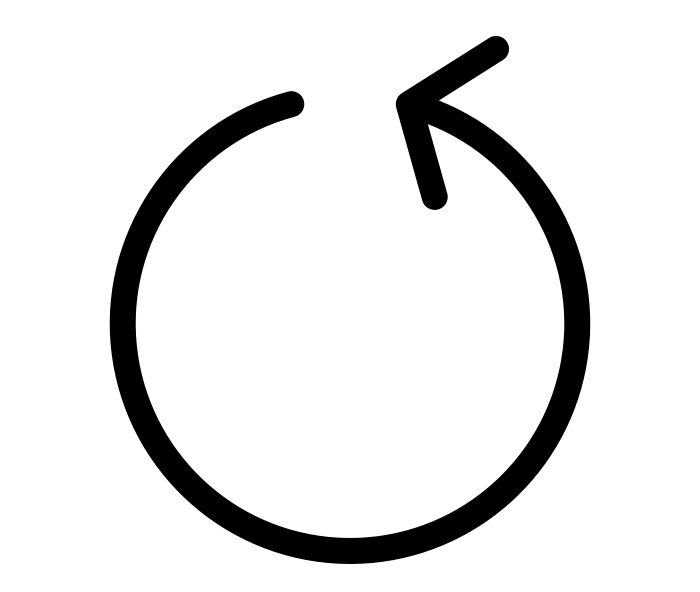
\includegraphics[width=1.8cm]{Images/2.png}
\\
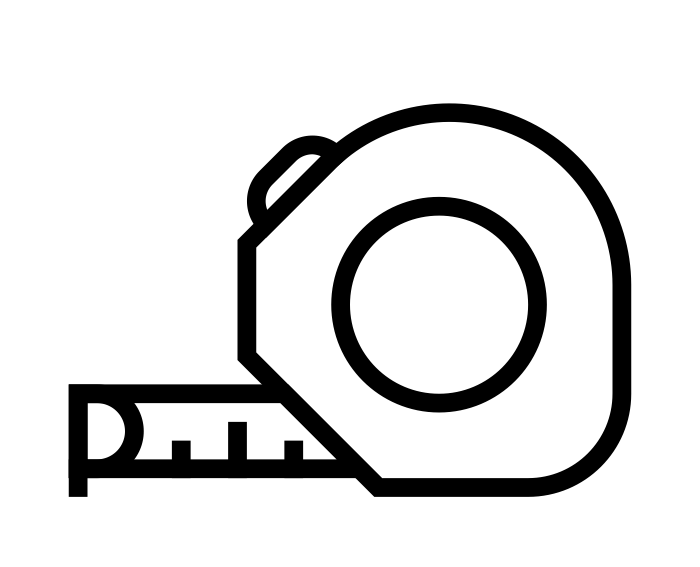
\includegraphics[width=1.8cm]{Images/3.png}
\\
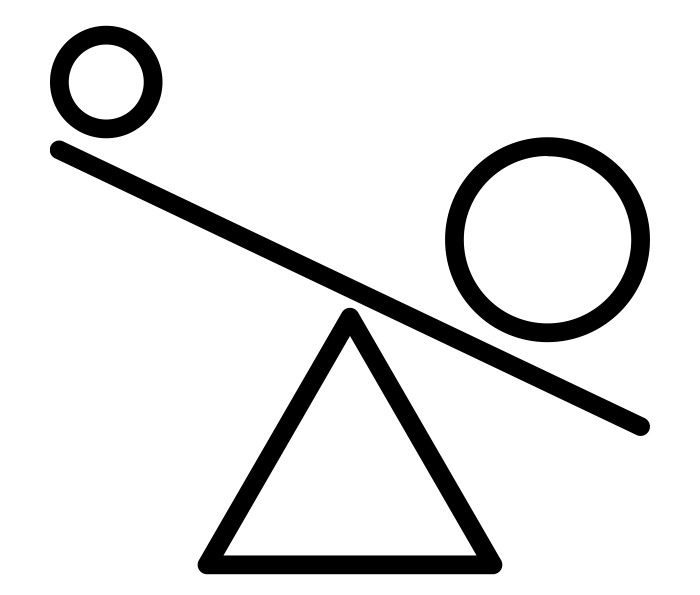
\includegraphics[width=1.8cm]{Images/4.png}
\\
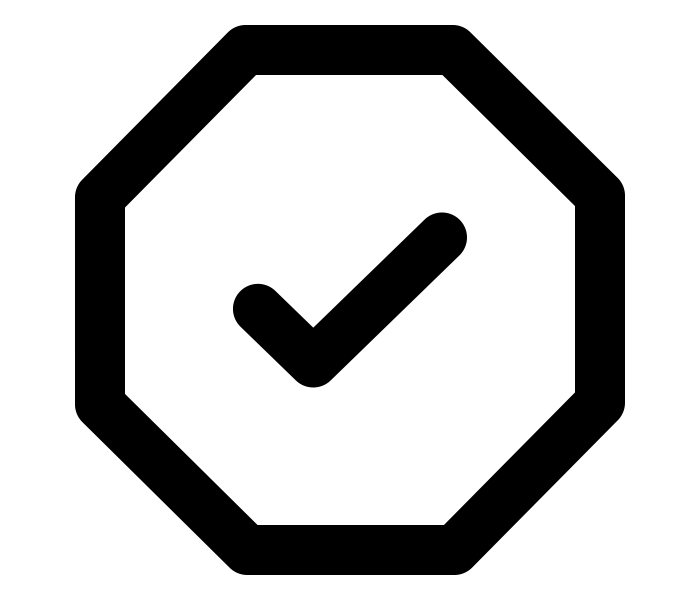
\includegraphics[width=1.8cm]{Images/5.png}
\end{column}
\end{columns}
\end{minipage}
\end{frame}


%%%%%%%%%%%%%%%%%%%%%%%%%%%%%%%%%%%%%%%%%%%%%%%%%%%%%%%%%%%%%%%%%%%%%%
\begin{frame}[fragile]{Conclusion}
\begin{minipage}[0.2\textheight]{\textwidth}
\begin{columns}[T]
\begin{column}{0.5\textwidth}
\begin{itemize}
\item Unremarkably, having total access to training data and having your adversary have no access to their own training data gives high control over test data predictions
\item Label-targeting attacks have good defenses, but not untargeted
\item Development of an untargeted defense seems like a trivial alteration to Neural Cleanse
\end{itemize}
\end{column}
\begin{column}{0.5\textwidth}
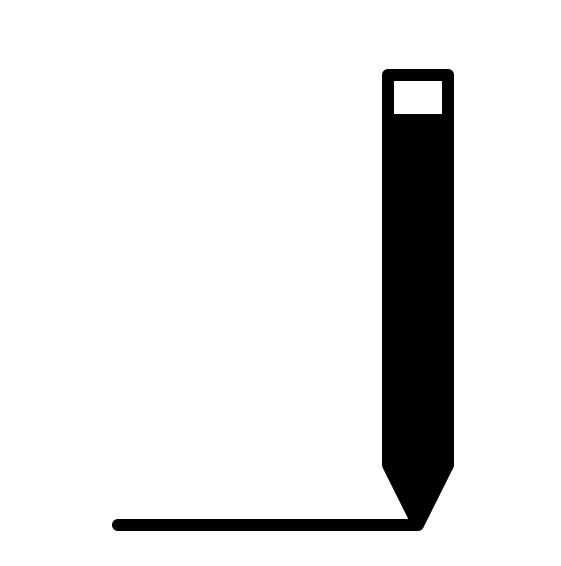
\includegraphics[width=5cm]{Images/conclusion.png}
\end{column}
\end{columns}
\end{minipage}
\end{frame}

\end{document}